\chapter{Windowing \& Fourier analysis}

\section{Spectral Leakage}

When performing a Fourier transform using a computer we must necessarily only transform a finite time-span $\tau$. The effect of this is the same as transforming the true, infinite signal multiplied by a unit top-hat function of width $\tau$. Transforming yields the true waveform convolved with a $\sinc$. If $\tilde{h}'(f)$ is the computed Fourier transform then
\begin{equation}
\tilde{h}'(f) = \intd{-\tau/2}{\tau/2}{h(t)\exp({2\pi i ft})}{t} = \left[\tilde{h}(f) \ast \tau \sinc(\pi f\tau)\right],
\end{equation}
where $\tilde{h}(f) = \mathscr{F}\left\{h(t)\right\}$ is the unwindowed Fourier transform of the infinite signal. This windowing of the data is a problem innate in the method, and results in spectral leakage.

\Figref{fig:Windowing-Rectangular} shows the computed Fourier transform for an example EMRB. The waveform has two distinct regions: a low-frequency curve, and a high-frequency tail. The low-frequency signal is the spectrum we are interested in; the high-frequency components are a combination of spectral leakage and numerical noise. The $\order{1/{f}}$ behaviour of the $\sinc$ gives the shape of the tail.\footnote{This has possibly been misidentified in figure 8 of \citet{Burko2007} as the characteristic strain for parabolic encounters.}
\begin{figure}%[!htp]
  \begin{center}
   \subfigure[Spectrum using no window. The calculated SNR is $\rho \simeq 12.5$.] {\label{fig:Windowing-Rectangular} 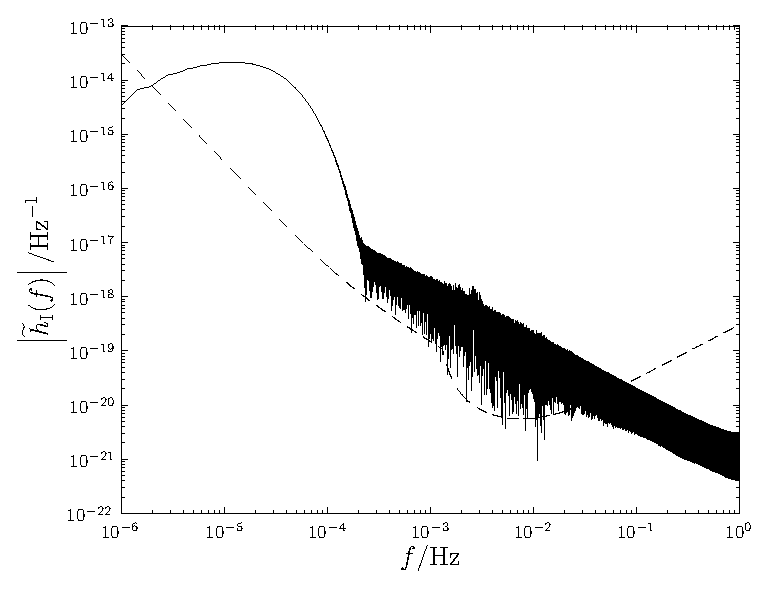
\includegraphics[width=0.475\textwidth]{./images/Fig_h_I_9_rectangular}} \quad
   \subfigure[Spectrum using a Nuttall window. The calculated SNR is $\rho \simeq 8.5$.] {\label{fig:Windowing-Nuttall} 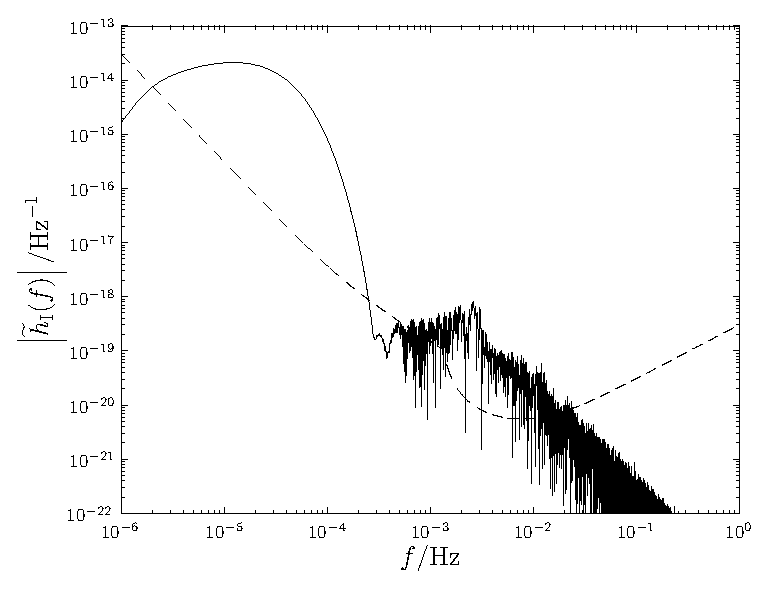
\includegraphics[width=0.475\textwidth]{./images/Fig_h_I_9_Nuttall}}
    \caption{Example spectra calculated using (a) a rectangular window and (b) Nuttall's four-term window with continuous first derivative \citep{Nuttall1981}. The spin of the MBH is $a_\ast = 0.5$, the mass of the orbiting CO is $\mu = 10 M_\odot$, the periapsis is $r\sub{p} = 50 r\sub{g}$ and the inclination is $\iota = 0.1$. The high-frequency tail is the result of spectral leakage. The level of the \textit{LISA} noise curve is indicated by the dashed line. The spectra are from detector I, but the detector II spectra look similar.\label{fig:Windowing}}
  \end{center}
\end{figure}

Despite being many orders of magnitude below the peak level, the high-frequency tail is still well above the noise curve for a wide range of frequencies. It therefore contributes to the evaluation of any inner products, and could mask interesting features. It is possible to reduce, but unfortunately not eliminate, the leakage using apodization: to improve the frequency response of a finite time series one can use a weighting window function $w(t)$ which modifies the impulse response in a prescribed way.

\section{Window functions}

The simplest window function is the rectangular (or Dirichlet) window $w\sub{R}(t)$; this is the top-hat described above. Other window functions are generally tapered.\footnote{When using a tapered window function it is important to ensure that the window is centred upon the signal; otherwise the calculated transform has a reduced amplitude.} There is a wide range of window functions described in the literature \citep{Harris1978,Kaiser1980,Nuttall1981,McKechan2010}. The introduction of a window function influences the spectrum in a manner dependent upon its precise shape. There are two distinct distortions: local smearing due to the finite width of the centre lobe, and distant leakage due to finite amplitude sidelobes. The window function may be optimised such that the peak sidelobe has a small amplitude, or such that the sidelobes decay away rapidly with frequency. Choosing a window function is a trade-off between these various properties, and depends upon the particular application.

For use with the parabolic spectra, the primary concern is to suppress the sidelobes. Many windows with good sidelobe behaviour exist; we consider three: the Blackman-Harris minimum four-term window \citep{Harris1978, Nuttall1981}
\begin{equation}
w\sub{BH}(t) = \sum_{n=0}^{3} a\super{BH}_n\cos\left(\frac{2n\pi t}{\tau}\right),
\end{equation}
where
\begin{equation}
%\begin{split}
a\super{BH}_0 = 0.35875, \quad a\super{BH}_1 = 0.48829, \quad
a\super{BH}_2 = 0.14128, \quad a\super{BH}_3 = 0.01168;
%\end{split}
\end{equation}
the Nuttall four-term window with continuous first derivative \citep{Nuttall1981}
\begin{equation}
w\sub{N}(t) = \sum_{n=0}^{3} a\super{N}_n\cos\left(\frac{2n\pi t}{\tau}\right),
\end{equation}
where
\begin{equation}
%\begin{split}
a\super{N}_0 = 0.355768, \quad a\super{N}_1 = 0.487396, \quad
a\super{N}_2 = 0.144232, \quad a\super{N}_3 = 0.012604,
%\end{split}
\end{equation}
and the Kaiser-Bessel window \citep{Harris1978, Kaiser1980}
\begin{equation}
w\sub{KB}(t;\beta) = \frac{I_0\left[\beta\sqrt{1 - (2 t/\tau)^2}\right]}{I_0(\beta)},
\end{equation}
where $I_\nu(z)$ is the modified Bessel function of the first kind, and $\beta$ is an adjustable parameter. Increasing $\beta$ reduces the peak sidelobe, but also widens the central lobe.

The Kaiser-Bessel window has the smallest peak sidelobe, but the worst decay ($1/f$); the Nuttall window has the best asymptotic behaviour ($1/f^3$); the Blackman-Harris window has a peak sidelobe similar to the Nuttall window, and decays asymptotically as fast (slow) as the Kaiser-Bessel window, but has the advantage of having suppressed sidelobes next to the central lobe.

Another window has been recently suggested for use with gravitational waveforms: the Planck-taper window \citep{Damour2000,McKechan2010}
\begin{equation}
w\sub{P}(t; \epsilon) = \begin{cases}
 {\displaystyle \recip{\exp(Z_+)+1}} & {\displaystyle \hphantom{\left(\recip{2} - \epsilon\right)}-\frac{\tau}{2} \leq t < -\tau\left(\recip{2} - \epsilon\right)} \\
 1 & {\displaystyle -\tau\left(\recip{2} - \epsilon\right) < t < \tau\left(\recip{2} - \epsilon\right)} \\
 {\displaystyle \recip{\exp(Z_-)+1}} & {\displaystyle \hphantom{-}\tau\left(\recip{2} - \epsilon\right) < t \leq \frac{\tau}{2}}
\end{cases},
\end{equation}
with
\begin{equation}
Z_\pm(t; \epsilon) = 2\epsilon\left[\recip{1 \pm 2(t/\tau)} + \recip{1 - 2\epsilon \pm 2(t/\tau)}\right].
\end{equation}
This was put forward for use with binary coalescences, and has superb asymptotic decay. However, the peak sidelobe is high, which is disadvantageous here. We therefore propose a new window function: the Planck-Bessel window which combines the Kaiser-Bessel and Planck-taper windows to produce a window which inherits the best features of both, albeit in a diluted form,
\begin{equation}
w\sub{PB}(t;\beta,\epsilon) = w\sub{P}(t; \epsilon)w\sub{KB}(t;\beta).
\end{equation}
The window functions' frequency responses are plotted in \figref{Response}.
\begin{figure}
  \begin{center}
  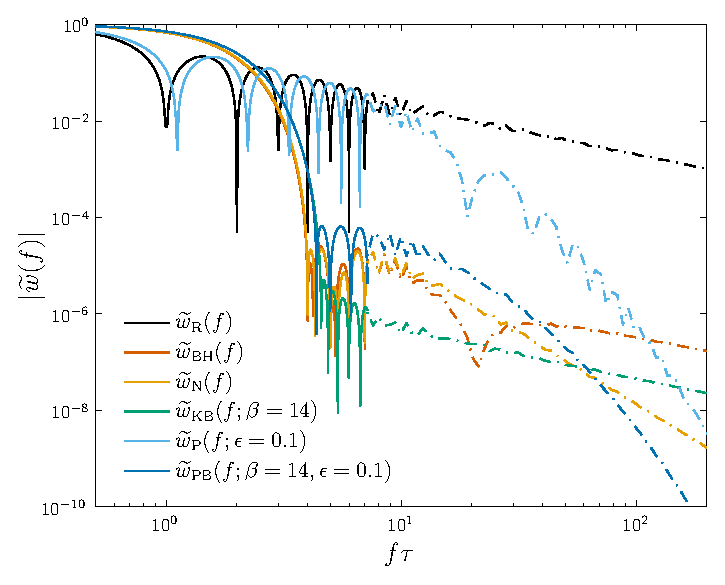
\includegraphics[width=0.6\textwidth]{./images/Fig_Response}
    \caption{Window function frequency response. To avoid clutter, the response function is only plotted in detail until $f\tau = 8$, above this a smoothed value is used, as indicated by the dot-dashed line. As well as having good asymptotic behaviour, the Planck-taper window has the narrowest main lobe, except for the rectangular window.}
    \label{fig:Response}
  \end{center}
\end{figure}
There is no window that performs best everywhere.

\Figref{Windowing} shows the computed Fourier transforms for an example EMRB using no window (alternatively a rectangular window), and the Nuttall window.\footnote{The Blackman-Harris, Kaiser-Bessel and Planck-Bessel windows give almost identical results.} Using the Nuttall window, the spectral leakage is greatly reduced; the peak sidelobe is lower, and the tail decays away as $1/{f^3}$ instead of $1/{f}$. The low frequency signal is not appreciably changed.

\section{Influence on results}

The choice of window function influences the results as it changes the form of $\widetilde{h}(f)$. The variation in results between windows depends upon the signal: variation is greatest for low frequency bursts, as then there is greatest scope for leakage into the detector band; variation is least significant for orbits with small periapses as then there are strong signals to relatively high frequencies, and spectral leakage is confined mostly to below the noise level. Preliminary investigations showed that the choice of window function (excluding the rectangular window) negligibly influences results for the closest orbits. As the periapse increases, such that the peak frequency decreases, differences begin to appear. To quantify the influence, we studied the diagonal elements of the Fisher matrix (\secref{Fisher}) from a selection of orbits about the GC with periapses ranging from $\sim 10 r\sub{g}$--$300 r\sub{g}$. For orbits with small periapses all five windows (excluding the rectangular window) produced very similar results: the Planck-taper window differed by a maximum of $\sim 0.5\%$ from the others, which all agreed to better than $0.1\%$. The worst case results came from the lowest frequency orbits (which extend beyond the range of detectability), then the Planck-taper window deviated by a maximum of $\sim 30\%$ in the value for the Fisher matrix elements, the Blackman-Harris deviated by $\sim 20\%$ and the others agreed to better than $\sim 5\%$. The Planck-taper window's performance is limited by its poor sidelobe behaviour; the Blackman-Harris is limited by its performance at high frequencies.

For this work we have used the Nuttall window. Its performance is comparable to the Kaiser-Bessel and Planck-Bessel windows, but it is computationally less expensive as it does not contain Bessel functions. Results should be accurate to a few percent at worst, and results from closer orbits, which provide better constraints, should be less affected by the choice of window function. We expect that any inaccuracies as a consequence of windowing are no greater than the error expected from using a numerical kludge approximation to generate the waveforms. Therefore, we are confident that none of our conclusions are sensitive to the particular windowing method implemented.